\documentclass[11pt,fleqn,twoside]{article}
\usepackage{makeidx}
\makeindex
\usepackage{palatino} %or {times} etc
\usepackage{plain} %bibliography style 
\usepackage{amsmath} %math fonts - just in case
\usepackage{amsfonts} %math fonts
\usepackage{amssymb} %math fonts
\usepackage{lastpage} %for footer page numbers
\usepackage{fancyhdr} %header and footer package
\usepackage{mmpv2} 
\usepackage{url}

\usepackage{graphicx}
\usepackage{algpseudocode}
\usepackage{multirow}
\usepackage{listings}
\usepackage{float}
\usepackage{caption}
\usepackage{subcaption}

% the following packages are used for citations - You only need to include one. 
%
% Use the cite package if you are using the numeric style (e.g. IEEEannot). 
% Use the natbib package if you are using the author-date style (e.g. authordate2annot). 
% Only use one of these and comment out the other one. 
\usepackage{cite}
%\usepackage{natbib}

\begin{document}

\name{Alexander D. Brown}
\userid{adb9}
\projecttitle{Kyffin Williams: Digital Analysis of Paintings}
\projecttitlememoir{Kyffin Williams: Digital Analysis of Paintings} %same as the project title or abridged version for page header
\reporttitle{Progress Report}
\version{0.4}
\docstatus{Draft}
\modulecode{CS39440}
\supervisor{Hannah M. Dee} % e.g. Neil Taylor
\supervisorid{hmd1}
\wordcount{?} %TODO

%optional - comment out next line to use current date for the document
%\documentdate{26th October 2011} 
\mmp

\setcounter{tocdepth}{3} %set required number of level in table of contents
\tableofcontents
\listoffigures
\listoftables

\newpage

\clearpage
%==============================================================================
\section{Project Summary}
%==============================================================================
Sir John ``Kyffin'' Williams was a landscape painter from Wales whose work was predominantly based 
in Wales and Patagonia. Gareth Lloyd Roderick, a PhD student in the National Library of Wales, has
collected data such as the date or location, of these paintings. This data allows for some 
interesting analysis; particularly that of temporal or geographical classification of a given 
painting. That is being able to take a painting and decide the year or location in which it was
painted from a database of existing, known, works by Kyffin Williams.

Temporal analysis will be the focus of this project as it allows for a diverse range of techniques;
from statistical analysis of colour values of the paintings to looking at the length and style of 
paintbrush strokes. Geographical analysis would likely be very difficult, especially as the locations
depicted were often sketched on-site then painted in a studio.

Whilst it would be nice to be able to predict the age of a painting with no known year, it is far
more interesting to try to guess the year of paintings for which the date is known. This project 
will use leave-one-out cross-validation to help measure the effectiveness and validity of the 
analysis techniques employed in this project. Leave-one-out validation can be used with this 
project as the data set is small enough not to incur large performance overheads and the overall
speed of the program is irrelevant so long as it completes within a decent amount of time.

One major limitation with this is it also includes the technique used for classification, some
techniques might work better with K-Nearest Neighbour whilst other might benefit from more complex
methods of classification. This means I will either have to stick with a single classification
algorithm and hope it's a good one for all techniques. Or I could find the best machine learning
technique for each individual analysis technique, then perform comparison. This does assume that
the best machine learning technique for every analysis technique exists within the scope of the
project.

As there has been a lot of research into this topic there is an introductory paper to the 
literature\cite{Stork2009Computer}, this paper specifies a lot of useful papers, including papers
like the \textsc{authentic} project\cite{Berezhnoy2005Authentic}.
%TODO Key Papers

Some examples of Kyffin Williams' work show the changes in his style over time; his early work as
shown in figure~\ref{fig:kyffin-early} often contained a lot of strokes and quite a lot of bright
colour. Comparing it to the work in around the middle of his career show in figure~\ref{fig:kyffin-mid}, there are visible differences;
the colours used are a lot darker and the strokes on the canvas are a lot more confident, leading
to a more ``blocky'' feel. His later work, shown in figure~\ref{fig:kyffin-late} retains this 
``blocky'' feel and the darker colours, but has a lot more detail like some of the paintings from
his earlier period.

There is also a period in 1969 where Kyffin Williams visited Patagonia and did quite a few works
in that area; these are visually very distinct as they use a lot of orange colours not common to
Welsh landscapes. Some of this work is shown in figure~\ref{fig:kyffin-patagonia}.

\begin{figure}[h]
\centering
\begin{subfigure}[b]{0.4\textwidth}
  \centering
  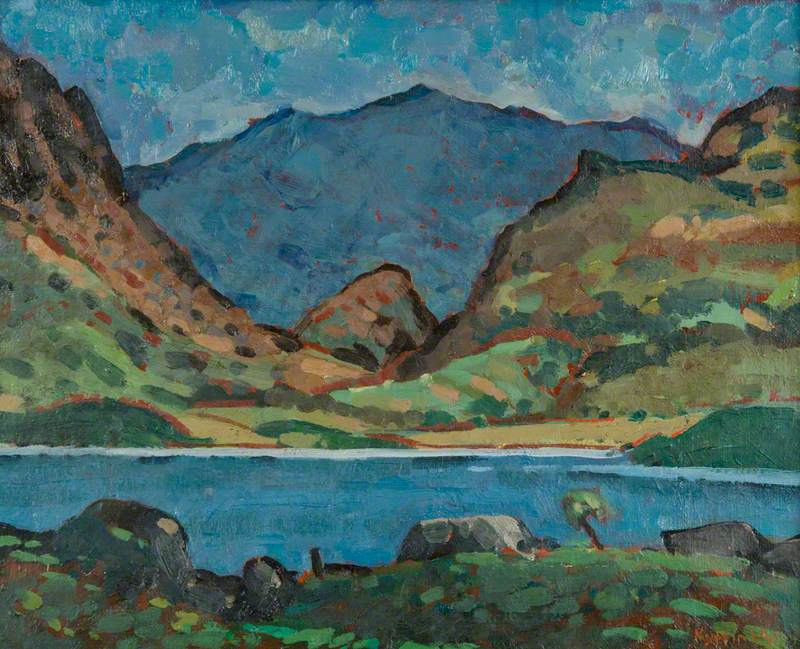
\includegraphics[width=\textwidth]{img/acnmw_acnmw_da006778_02_large.jpg}
  \caption{Snowdon from Llyn Nantle (1945)}
\end{subfigure}
\begin{subfigure}[b]{0.4\textwidth}
  \centering
  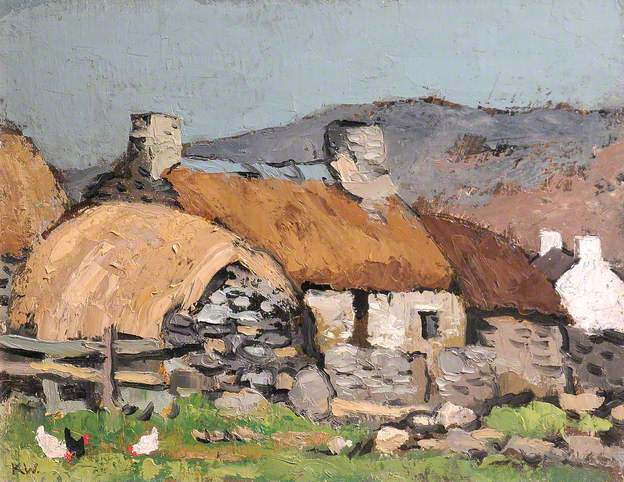
\includegraphics[width=\textwidth]{img/nwm_oym_1_90_624x544.jpg}
  \caption{Swtan (1947)}
\end{subfigure}
\caption{Early works by Kyffin Williams}
\label{fig:kyffin-early}
\end{figure}

\begin{figure}[h]
\centering
\begin{subfigure}[b]{0.4\textwidth}
  \centering
  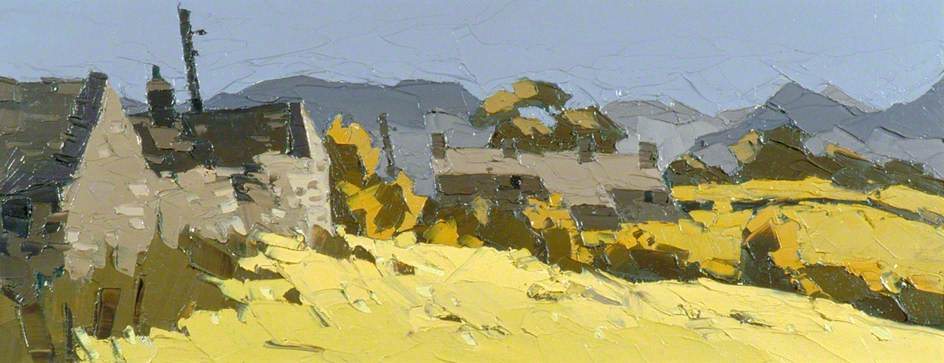
\includegraphics[width=\textwidth]{img/gac_gac_13839_large.jpg}
  \caption{Nant Ffrancon from Llandegfan (1970)}
\end{subfigure}
\begin{subfigure}[b]{0.4\textwidth}
  \centering
  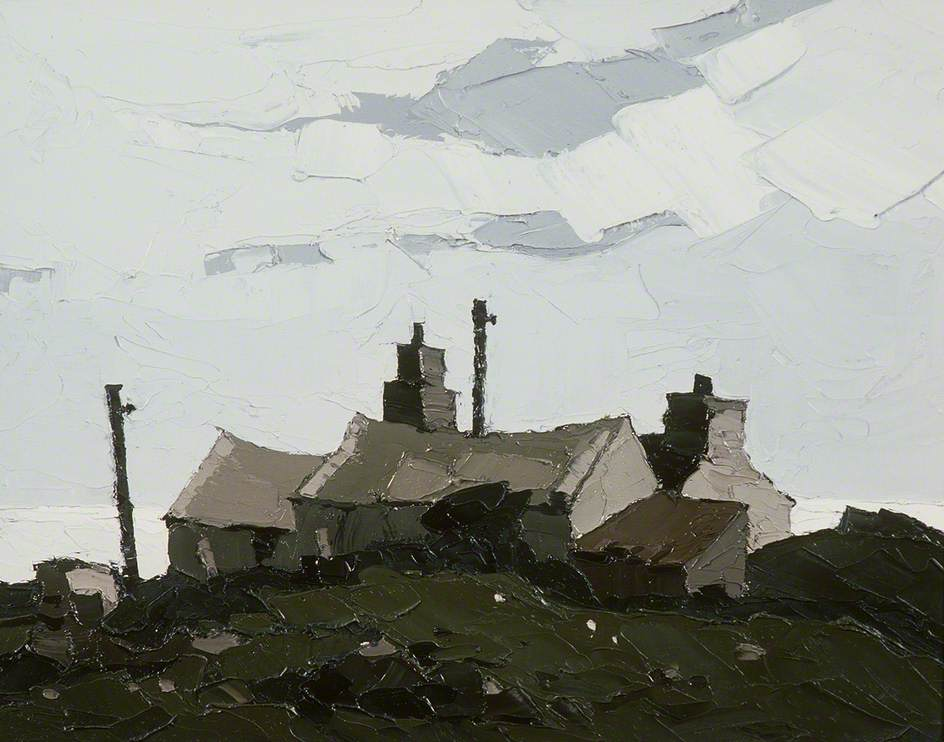
\includegraphics[width=\textwidth]{img/nlw_nlw_gcf02283_large.jpg}
  \caption{Farm, Llanfairynghornwy (1974)}
\end{subfigure}
\caption{Works by Kyffin Williams in the middle of his career}
\label{fig:kyffin-mid}
\end{figure}

\begin{figure}[h]
\centering
\begin{subfigure}[b]{0.4\textwidth}
  \centering
  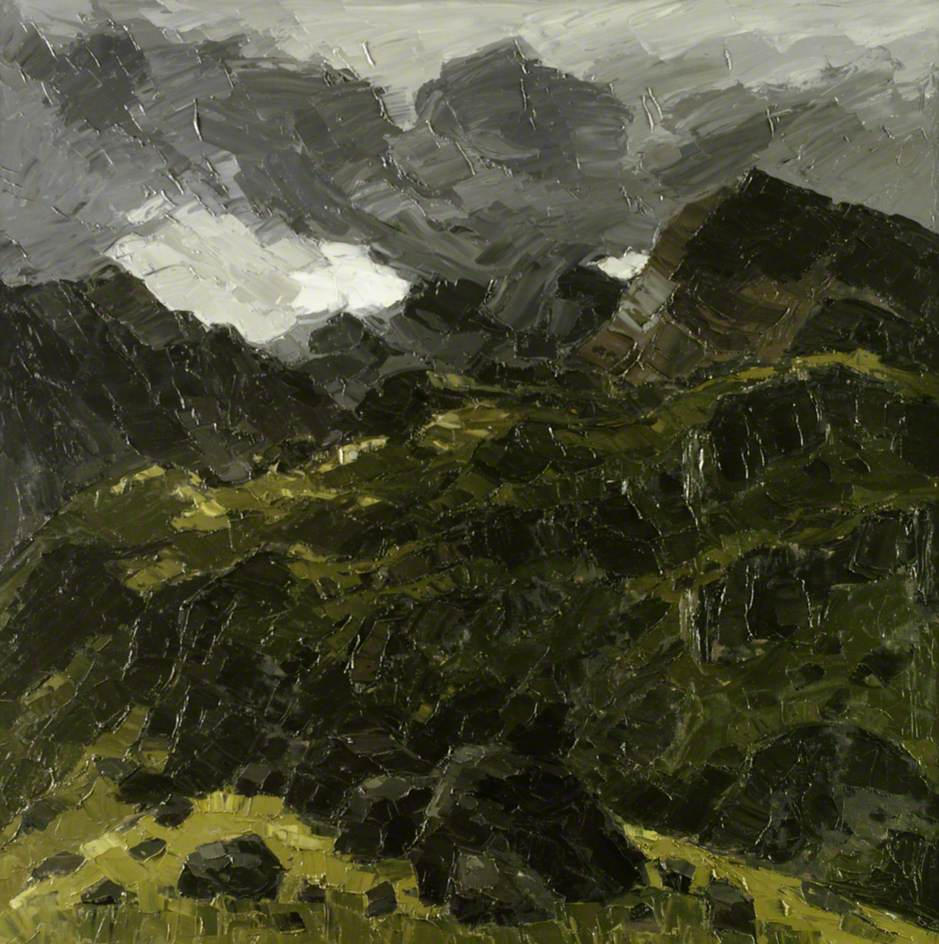
\includegraphics[width=\textwidth]{img/nlw_nlw_gcf06690_large.jpg}
  \caption{Pengwyryd (1999)}
\end{subfigure}
\begin{subfigure}[b]{0.4\textwidth}
  \centering
  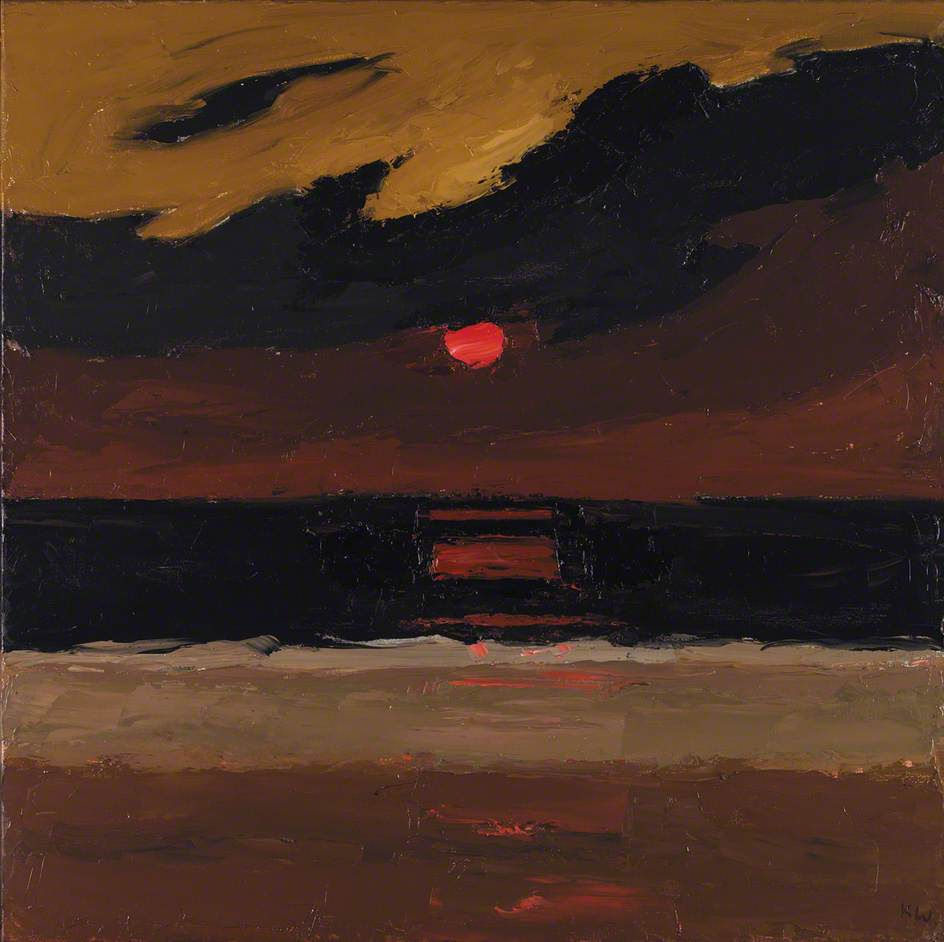
\includegraphics[width=\textwidth]{img/nlw_nlw_gcf08104_large.jpg}
  \caption{Sunset, Anglesey (2004)}
\end{subfigure}
\caption{Works by Kyffin Williams towards the end of his career}
\label{fig:kyffin-late}
\end{figure}

\begin{figure}[h]
\centering
\begin{subfigure}[b]{0.4\textwidth}
  \centering
  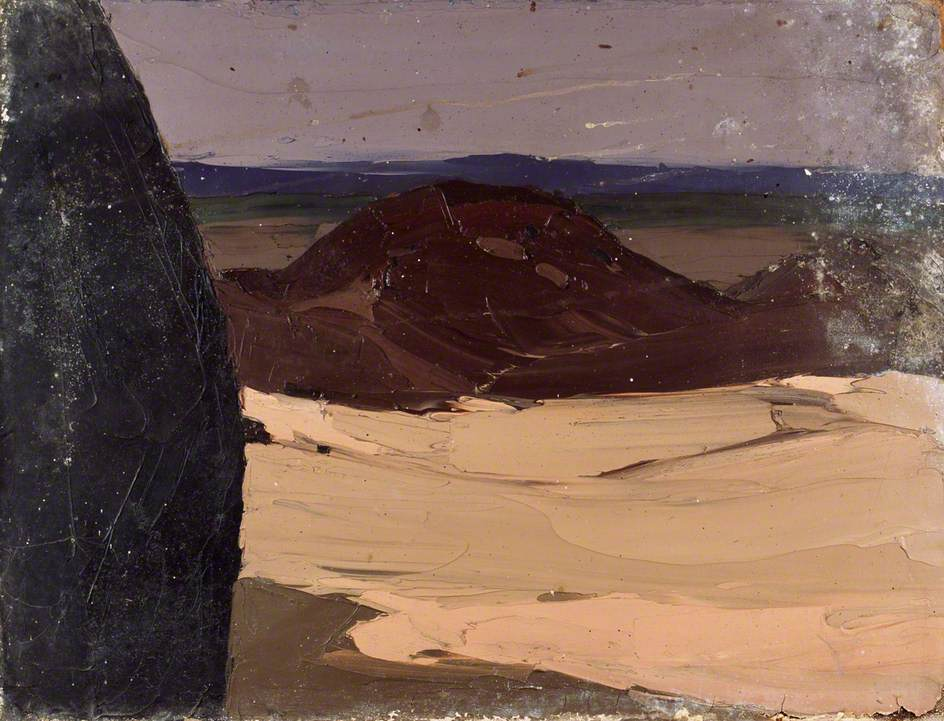
\includegraphics[width=\textwidth]{img/nlw_nlw_kwf00325_large.jpg}
  \caption{Paith, Patagonia (1969)}
\end{subfigure}
\begin{subfigure}[b]{0.4\textwidth}
  \centering
  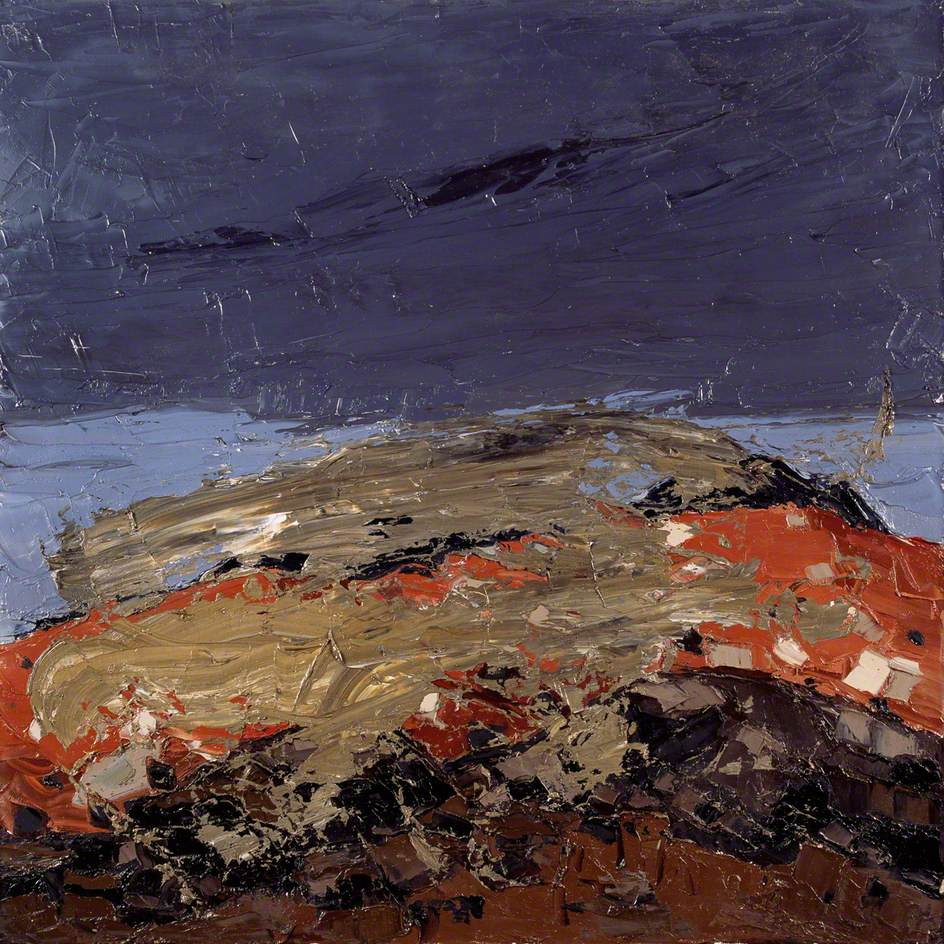
\includegraphics[width=\textwidth]{img/nlw_nlw_kwf00103_large.jpg}
  \caption{Patagonian Landscape (1969)}
\end{subfigure}
\caption{Works by Kyffin Williams from his trip to Patagonia}
\label{fig:kyffin-patagonia}
\end{figure}

At current I have had one meeting with both Lloyd and Hannah to discuss the current progress of 
the project and where we see the project progressing to. Lloyd was impressed by the current state
of the project and was looking forward to see where it was leading to.

We also discussed the potential of getting a paper published out of this project.

\clearpage
%==============================================================================
\section{Current Progress}
%==============================================================================

At current, there are three main areas in which progress has been made:

\begin{itemize}
\item Research into tools.
\item Research into related work.
\item Progress in development and experimentation.
\end{itemize}

\clearpage
%==============================================================================
\subsection{Research into tools}
%==============================================================================

\subsubsection{Library and Language Research}
The first step in the project was to research into the numerous image processing/computer vision
libraries available for use with the aim to find the most suitable library to use constantly for 
the rest of the project. Because of this the library had to be easy to install and use, as well as
having all the necessary features which would be used in this project.

The choice of library also has a knock-on affect on the choice of language this project would be 
written in. To this end I downloaded each of the libraries in turn, created a simple application to
 perform blur on a single image to test their use and documentation. From this I gained a good 
insight into how easy that library would be to perform more complex tasks and how confident I felt 
with the language(s) the library has bindings for.

Table~\ref{tab:libraries-overview} shows an overview of all the libraries I have currently 
considered and experimented with.

\begin{table}[h]
\begin{tabular}{| c | c | c | c | c | c | c |}
								  \hline
\multirow{2}{*}{\textbf{Library}}	& \multicolumn{4}{|c|}{\textbf{Platform}}			& \multirow{2}{*}{\textbf{Language(s)}}	& \textbf{Example}	\\\cline{2-5}
					&  Windows	& Mac 		& Linux 	& Android	&					&			\\\hline
OpenCV					& \checkmark	& \checkmark	& \checkmark	& \checkmark	& C, C++, Python			& Figure~\ref{fig:opencv}\\\hline
FIJI					& \checkmark	& \checkmark	& \checkmark	& 		& Java					& Figure~\ref{fig:fiji}	\\\hline
IVT					& \checkmark	& \checkmark	& \checkmark	& 		& C++					& Figure~\ref{fig:ivt}	\\\hline
VXL					& \checkmark	& \checkmark	& \checkmark	& 		& C++					& Figure~\ref{fig:vxt}	\\\hline
\end{tabular}
\caption{Comparison of image processing/computer vision libraries.}
\label{tab:libraries-overview}
\end{table}

Of these libraries OpenCV was the easiest to work with. OpenCV also boasts a wide range of 
features, all of which are well documented. FIJI provided a lot of high-level functionality, but
for use as a library it quickly became unwieldy and was difficult to find the correct classes just 
for the simple task of blurring an image. On a side note, I only managed to get the blurring 
outputting a greyscale image in the short period of time I spent using FIJI.

IVT was somewhat similar to FIJI in that it had a good range of high-level features, but was less
impressive as a library. Despite following the example code I struggled to compile my own example
and eventually gave up trying to get a working binary due to time constraints.

%TODO Actually use VXL and then write about it.

Having weighed up these libraries I it became fairly apparent that OpenCV would be the best choice,
not only did it act as an easy to use library, it is also seems that is is one of the most 
prevalent libraries for Computer Vision. For the Kyffin Williams project OpenCV provides a lot of
pre-built helpers which allow for very rapid production of the early elements of the project. For
example it is able to handle loading images in different colour spaces, generating histograms of
images and even comes with its own machine learning libraries.

Having decided to go with OpenCV I was then faced with a choice of languages. OpenCV runs natively
with C++ and has bindings for Python. Of these two languages I am slightly more familiar with C++ 
and I am also used to the syntax from programming Java continually for three years. 

However, I wanted to take a rapid prototyping approach with this project; constantly adding new 
modules each week to build up a better and better system. C++ seemed too heavyweight for this 
approach, whilst Python seemed designed for it.

Another consideration I had was that the results of any analysis could take any form at all, from
an array of numbers to a complex data structure returned by OpenCV. Trying to work around this with
a statically typed language such as C++ could end up being difficult, especially when trying to 
keep a object-orientated approach. With a dynamically typed language such as Python it's a lot 
easier to pass these sorts of objects so long as the functions you pass to are expecting the right 
sort of object.

There may be some parts of the project which I might consider writing in C++ after prototyping in 
Python. An example of this would be if I wrote an algorithm which located strokes across the 
painting, as it may be used in other projects, not just my own.


\begin{figure}[p]
\begin{lstlisting}[language=Python]
import cv

im = cv.LoadImageM("tux.png")
blur = cv.CreateMat(im.rows, im.cols, im.type)
cv.Smooth(im, blur, cv.CV_BLUR, 9)
cv.SaveImage("tux_blurred_opencv.png", blur)
\end{lstlisting}
\caption{Using OpenCV to blur an image}
\label{fig:opencv}
\end{figure}

\begin{figure}[p]
\begin{lstlisting}[language=Java]
package fiji;

import ij.IJ;
import ij.io.FileSaver;
import imagescience.feature.Smoother;
import imagescience.image.ColorImage;
import imagescience.image.Image;

public final class Blur {
	public static final String IMG_PATH = "tux.png";
	public static final String OUTPUT_PATH = "tux_fiji.png";

	public static void main(String[] args) {
		final Image image = new ColorImage(IJ.openImage(IMG_PATH));
		final Smoother s = new Smoother();
		final Image blurred = s.gauss(image, 9f);
		final FileSaver fs = new FileSaver(blurred.imageplus());
		fs.saveAsPng(OUTPUT_PATH);
	}
}
\end{lstlisting}
\caption{Using FIJI to blur an image}
\label{fig:fiji}
\end{figure}

\begin{figure}[p]
\begin{lstlisting}[language=C++]
#include <stdio.h>
#include "Image/ByteImage.h"
#include "Image/ImageProcessor.h"

int main(int argc, char **argv) {
	CByteImage in;
	CByteImage out;
	char* from = "tux.png";
	char* to = "tux_ivt.png";

	in.LoadFromFile(from)
	out = CByteImage(in);
	ImageProcessor::GaussianSmooth(&in, &out, 1.0f, 3);
	out.SaveToFile(to)
}
\end{lstlisting}
\caption{Using IVT to blur an image}
\label{fig:ivt}
\end{figure}

\begin{figure}[p]
\caption{Using VXT to blur an image}
\label{fig:vxt}
\end{figure}

\subsubsection{Other Tools}
Having used git for several personal projects I was keen to continue using it for my version 
control system. GitHub was a convenient hosting company to go with as they provide students with 
free private repositories and have very high uptime. It also means I am able to easily work on any 
system without difficulty but with the assurance of security. This is preferable to hosting my own
repositories and running the risk of losing a lot of work.

Git is one of the nicer version control programs I have used and has some nice extensions (shell
integration with zsh, git-flow for helping with the development process) and its decentralised 
nature allows me to easily work where-ever I feel most comfortable.

\clearpage
%==============================================================================
\subsection{Research into Existing Work}
%==============================================================================

\subsubsection{Research into Stroke Analysis}
Stroke analysis is one of the main goals for this project. It is quite apparent from looking at 
Kyffin Williams' paintings that his brushstrokes change over time, his early work having lots of
smaller strokes over the canvas to large bold strokes in his later work.

The first paper I found relating to the analysis of brushstrokes involved moving a circular filter
across the whole painting to find the ridges of strokes, then to fill any unbroken areas. They then
shrunk these areas to a single pixel line and fitted a $n^{\text{th}}$ order polynomial to this
line\cite{Berezhnoy2005Authentic}. This method seems fairly simplistic, but could be an interesting
first step, but as it is more focused on authenticating paintings it may be of limited use.

Another method for stroke analysis has been published in the IEEE Transactions on Pattern Analysis
and Machine Learning journal. This method is far more complex, but is able to extract and label
individual brushstrokes. An interesting part of their findings was the ability to date some of Van
Gogh's paintings to a known period in his career\cite{Li2012Rhythmic}.

\clearpage
%==============================================================================
\subsection{Progress in Development and Experimentation}
%==============================================================================

\subsubsection{Design}
\begin{figure}[H]
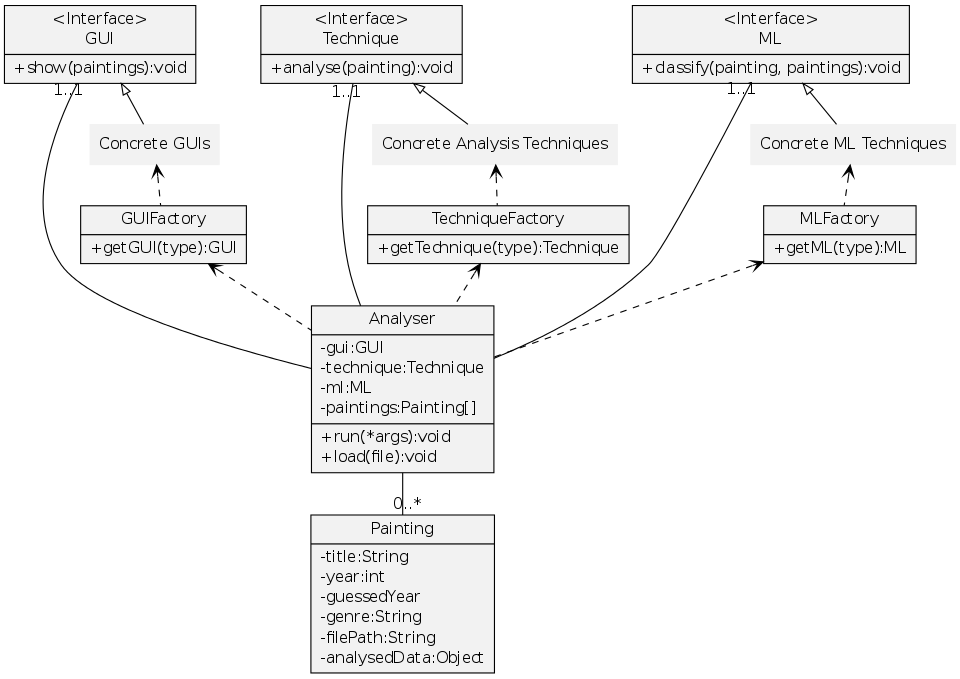
\includegraphics[scale=0.5]{img/design.png}
\caption{Initial Design}
\label{fig:init-class}
\end{figure}

An initial UML class diagram is depicted by figure~\ref{fig:init-class}. This design will allow 
additional techniques, both analysis and machine learning based, to be added easily. Command line
arguments, or later a GUI front-end, will be used to specify which techniques should be used.

The GUI elements depicted are used for visualising the analysed data or results of the machine
learning algorithms. An example of this is a graphical representation of the colour space averages
(see figure~\ref{fig:mean-hsv-by-year}).

\subsubsection{Colour Space Statistical Analysis}
With the design solidified, I began to work on the statistical analysis of digital images. The 
easiest of these techniques is to read the image pixel by pixel, taking the various intensities at
that pixel, then averaging them out over the whole image.

The most common colour space used is RGB (Red, Green, Blue), where each pixel holds three different
intensities, one for each colour with a value of 0 to 255.

Using this analysis I plotted a graph of all paintings with a known year against the different 
intensities (see figure~\ref{fig:mean-rgb-by-year}). Whilst the RGB values do all slowly increase
over time and particularly the Red and Green values, the change may not be enough to classify new
examples due to the fluctuations in the data. 

\begin{figure}[p]
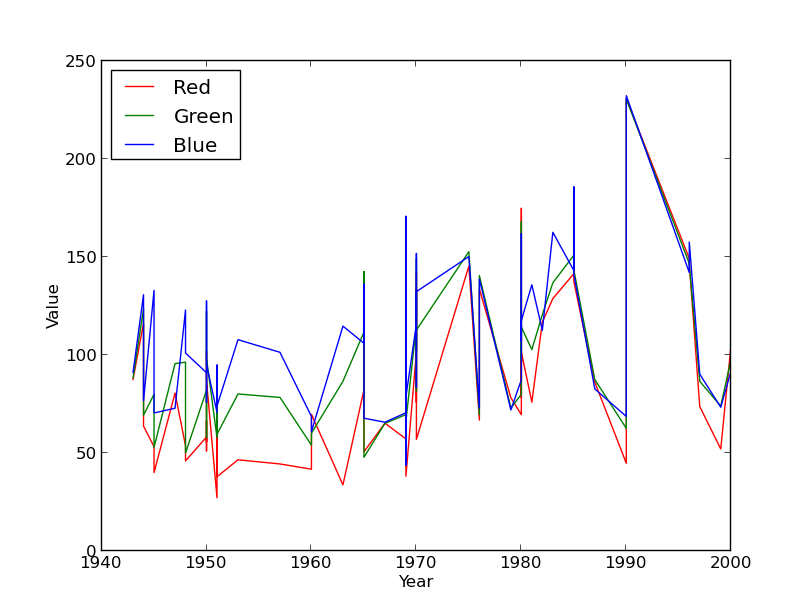
\includegraphics[scale=0.5]{img/kyffin-rgp-avg.png}
\caption{Mean RGB intensities by year.}
\label{fig:mean-rgb-by-year}
\end{figure}

Another popular colour space used in image processing is HSV (Hue, Saturation, Value) as it shows
variations in colour, saturation and brightness separately (unlike RGB where all three values are
affected by changes in brightness). It was a simple matter of changing the existing code for RGB
so that it would analyse HSV values instead.

Figure~\ref{fig:mean-hsv-by-year} shows a similar graph to the one in
figure~\ref{fig:mean-rgb-by-year} only with HSV colour space instead of RGB. With this the Hue 
stays roughly the same throughout, whilst the saturation slowly declines and the value increases;
this would make the colours brighter but with less colour to them. Whilst the reduction of colour
over time is fairly obvious looking at Kyffin Williams' work, the increase in brightness was not
something I would have necessarily have picked up on.

It's also quite interesting that both of these graphs has a dip during the Patagonia period, though
both do have quite a high variance, meaning classification will tend to be unreliable. HSV does 
seem slightly less so than RGB.

\begin{figure}[p]
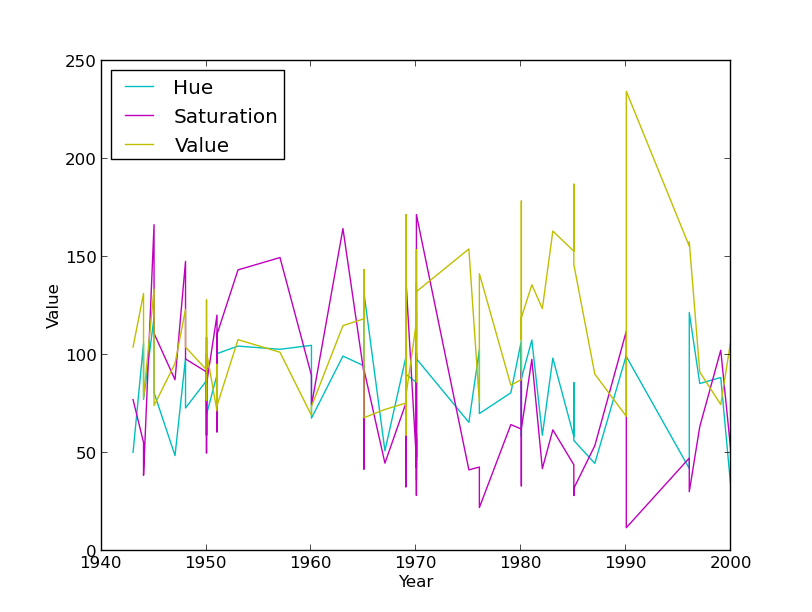
\includegraphics[scale=0.5]{img/hsv-legend-12-11-01.png}
\caption{Mean HSV intensities by year. Note: value increases as time progresses showing Kyffin
Williams' paintings became brighter as time went on.}
\label{fig:mean-hsv-by-year}
\end{figure}


\subsubsection{Histogram Analysis}
With colour-space analysis complete, the next sensible step was to start generating colour 
histograms from Kyffin Williams paintings.

A histogram is a nice way of representing the distribution of colour in a given image and is 
therefore a richer representation of a painting than colour-space averages.

As with before, histograms can be taken from different colour spaces, currently only the program
can only generate RGB histograms (shown in figure~\ref{fig:histogram}), but it is trivial to 
include HSV histograms too.

\begin{figure}[h]
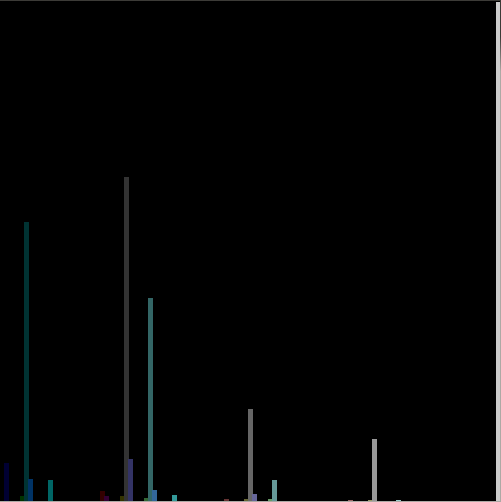
\includegraphics[scale=0.5]{img/histogram.png}
\caption{Example of an RGB Histogram.}
\end{figure}

From looking at the RGB histograms it becomes very apparent that Red is a very rare colour in 
isolation, except during the Patagonia period. Similarly green in isolation appears infrequently,
where it is visible it's usually more of a teal colour. Very bright colours are also rare except
in paintings with a lot of (Welsh) sky.

\subsubsection{Nearest Neighbour Classification}
Having looked at different representations of colour in paintings, the next part was to create a 
simple classification algorithm. The simplest of which is 1-Nearest Neighbour, that is; take the 
``Nearest'' training example to the example to be classified and classify the year of this example 
with the year of the nearest example (see figure~\ref{fig:1-nn}).

This simple algorithm can be expanded to be a K-Nearest Neighbour algorithm without too much effort
(see figure~\ref{fig:k-nn}). Instead of storing a single nearest neighbour you can simply store a
list of them (making 1-Nearest Neighbour still work without issue) and then have some small amount
of processing at the end to get a hold of the best neighbour. This processing will likely take the
form of a simple statistic method such as the mean or the modal year.

\begin{figure}[h]
\begin{algorithmic}
\State $bestDistance \gets \infty$
\For{$x = 1 \to X$}
	\If{$distance(a, x) < bestDistance$}
		\State $bestDistance \gets distance(a, x)$
	\EndIf
\EndFor
\end{algorithmic}

Where:\\
\(a\) is the example to classify.\\
\(X\) is the list of all training examples.
\caption{1-Nearest Neighbour}
\label{fig:1-nn}
\end{figure}

\begin{figure}[h]
\begin{algorithmic}
\State $kBest \gets []$
\For{$x = 1 \to X$}
	\State $cur \gets distance(a, x)$
	\For{$k = 1 \to K$}
		\If{$cur < kBest[k]$}
			\State $temp \gets kBest[k]$
			\State $kBest[k] \gets cur$
			\State $cur \gets temp$
		\EndIf
	\EndFor
\EndFor
\end{algorithmic}
Where:\\
$a$ is the example to classify.\\
$X$ is the list of all training examples.
$K$ is the number of nearest neighbours to check.
\caption{K-Nearest Neighbour}
\label{fig:k-nn}
\end{figure}


\subsubsection{Distance Measures}
Working out the ``Nearest'' example to a given painting requires some way of measuring distance
between the two.

One very simple way of doing this is Manhattan distance (equation~\ref{eq:manhattan}). This distance
measure can be improved further to Euclidean distance (equation~\ref{eq:euclidean}) without too much
effort. There are numerous other methods of measuring the distance of points in space, including
those which focus on the distance between colour histograms, however Euclidean and Manhattan 
distance are both good starting points.

\begin{figure}[h]
\[
d = \sum^X_{x=0}{|a_x - b_x|}
\]

\(X\): All dimensions present in both \(a\) and \(b\).\\
\(a\): The first point.\\
\(b\): The second point.

\caption{Manhattan Distance}
\label{eq:manhattan}
\end{figure}

\begin{figure}[h]
\[
d = \sqrt{\sum^X_{x=0}{(a_x - b_x)^2}}
\]

\(X\): All dimensions present in both \(a\) and \(b\).\\
\(a\): The first point.\\
\(b\): The second point.
\caption{Euclidean Distance}
\label{eq:euclidean}
\end{figure}



\subsubsection{Leave-one-out Cross Validation}
\begin{figure}[h]
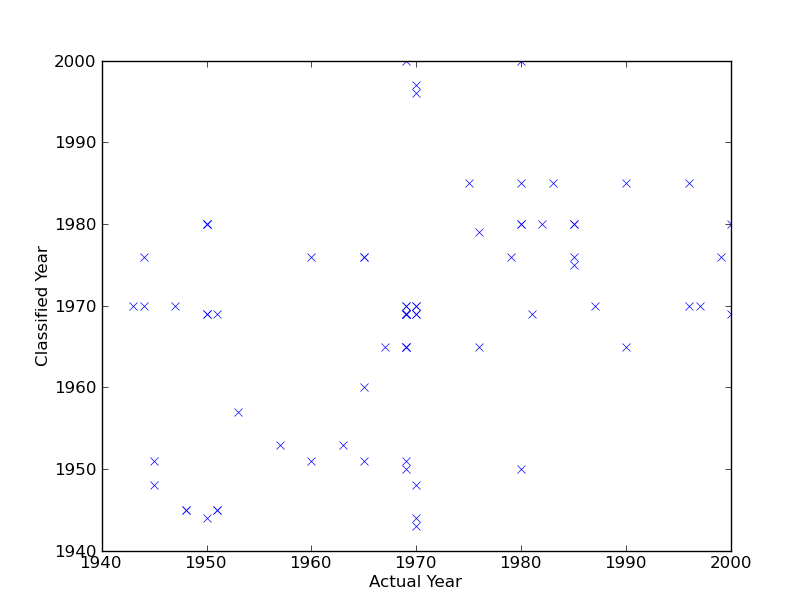
\includegraphics[scale=0.5]{img/validation-rgb-1nn.png}
\caption{Leave-one-out cross validation of actual year against classified year using RGB statistical analysis and
1-nearest neighbour classification.}
\label{fig:validation-rgb-1nn}
\end{figure}

The idea of leave-one-out cross validation is to take the entire training set, remove a single 
example and then to classify this example against the rest of the training set. You can then do
this for every example in the training set and be able to plot a graph of the actual year against
the classified year, aiming for the line $x=y$, an example of this is shown in 
figure~\ref{fig:validation-rgb-1nn}. With this information we can also work out the correlation 
between the two and have an indication of how each analysis technique performs.


\subsection{Technical Issues}
Having engineered software before I know that the biggest issue with developing a piece of software
is working with external APIs. With this project I can currently get away with only having to work
with a few APIs; OpenCV being the main candidate. I have had some struggles trying to understand
exactly what the API wants as inputs and returns as outputs, but that is more due to a slight lack
of knowledge in the area of computer vision and image processing rather than the API being complex.

I am currently reading up on image processing and computer vision, using free,
online resources\cite{Prince2012Computer} and knowledge within the department.

OpenCV seems like a good library to work with, though I have yet to use it for any
specialised image processing (i.e. I have only used built-in methods OpenCV provides by default).
I currently don't see any issue as the python bindings for OpenCV use numpy in the background. Both
of these libraries are widely used and open source. If I do happen to have any problems with either
of these libraries there is a substantial community behind them and the option to fix any problems
and give them back to the projects.

Another technical issue associated with this project is the resolution of the paintings in the 
current database. Most of the images are fairly small as they are intended to be used on a website
rather than in an image processing application. There is potential that I may be able to get a hold
of larger images for certain paintings, but if the techniques could be made to work on the current
size of image it would probably be better for the project as a whole.

A problem associated with this is memory limits; for smaller images only a small amount of data
will need to be stored, but for more complex techniques, large matrices may be generated and memory
might become a precious resource. At current all analysis is run before classification but it may
be necessary to only hold the analysis data for the current example to classify and the training 
example for which we are currently measuring the distance to. This would not be a difficult change
to make, but may slow the program down as a whole.

\clearpage
%==============================================================================
\section{Planning}
%==============================================================================

\subsection{Methodology}
The methodology I am taking as part of this project is a mix of iterative development with rapid
prototyping. I think this approach will work well for this project as it is built up of a lot of 
small, isolated modules which perform discrete tasks.

Other models of development would likely slow the development of each of these modules down and are
therefore less appropriate for this project. Some agile methodologies may also be a good approach,
but as most agile methodologies are designed for teams rather than individual projects they are
inappropriate.

Figure~\ref{fig:gantt} depicts the Gantt chart I am going to try to follow for the course of this
project.


\clearpage
\newpage
\subsection{Gantt Chart}
\begin{figure}[H]
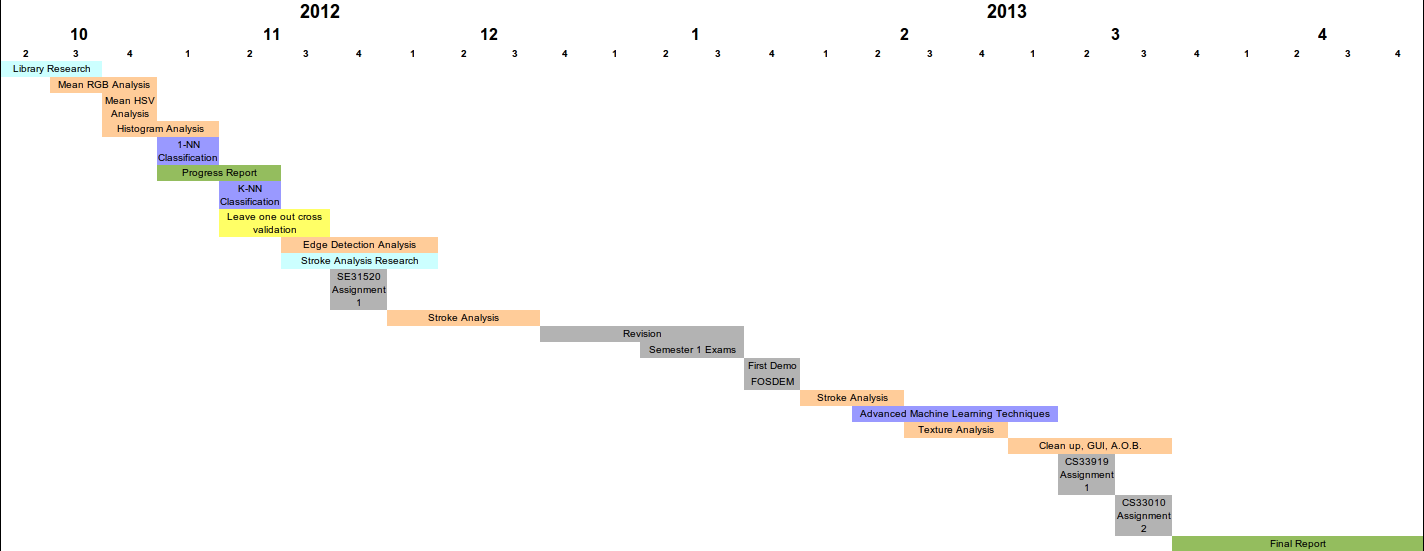
\includegraphics[scale=0.45, angle=90]{img/gantt.png}
\caption{Gantt Chart for the Kyffin Williams project}
\label{fig:gantt}
\end{figure}

\clearpage
\subsection{Mid-term Demonstration}
For the mid-term demonstration I aim to be able to demonstrate
%TODO


%
%You need to include an annotated bibliography. This should list all relevant web pages, books, journals etc. that you have consulted in researching your project. Each reference should include an annotation. 

%The purpose of the section is to understand what sources you are looking at.  A correctly formatted list of items is sufficient. You might go further and make use of bibliographic tools, e.g. BibTeX in a LaTeX document, could be used to provide citations, for example \cite{NumericalRecipes} \cite{MarksPaper} \cite[99-101]{FailBlog} \cite{kittenpic_ref}.  The bibliographic tools are not a requirement, but you are welcome to use them.   

%You can remove the above {\em Your Bibliography} section heading because it will be added in by the renewcommand which is part of the bibliography. The correct annotated bibliography information is provided below. 
%
% End of comment out / remove the lines. They are only provided for instruction for this example template. 
%


\nocite{*} % include everything from the bibliography, irrespective of whether it has been referenced.

% the following line is included so that the bibliography is also shown in the table of contents. There is the possibility that this is added to the previous page for the bibliography. To address this, a newline is added so that it appears on the first page for the bibliography. 
\newpage
\addcontentsline{toc}{section}{Annotated Bibliography} 

%
% example of including an annotated bibliography. The current style is an author date one. If you want to change, comment out the line and uncomment the subsequent line. You should also modify the packages included at the top (see the notes earlier in the file) and then trash your aux files and re-run. 
%\bibliographystyle{authordate2annot}
\bibliographystyle{IEEEannot}
\renewcommand{\refname}{Annotated Bibliography}  % if you put text into the final {} on this line, you will get an extra title, e.g. References. This isn't necessary for the outline project specification. 
\bibliography{mmp} % References file


\end{document}
